\chapter{Test Results}
\label{cha:pierwszyDokument}

\section{First Set of Tests}

First set of tests uses historical data from year 2009 (data of 3 different stocks have been used). 
Portfolio contained 3 assets:

\begin{itemize} 
  \item KGHM
  \item TPSA
  \item PKO
\end{itemize}

Multi-agent platform has been used to run algorithms .
It was configured in the following way: 

\begin{itemize}
  \item configured to simulate trading strategy throughout the entire year 2009
  \item migration mechanism between Computing Nodes has been enabled
  \item two Computing Nodes (with appropriate algorithms) has been used to gather results
\end{itemize}

Trend following algorithm has been tested without multi-agent running platform as it is a standalone R script.

\subsection{Trend Following}

\subsubsection{Short-term trend results}

As described in \ref{trend_following_impl} and \ref{sec:trendFollowing}, we can adjust our trading rules to seek out short-term trends
 (by changing the values of $N$ and $M$ in the \emph{Simple Moving Average} method).
With values $N = 10$, $M = 20$ the SMA method focused on short-term trends.
 

\begin{figure}[H]
  
  \begin{center}
    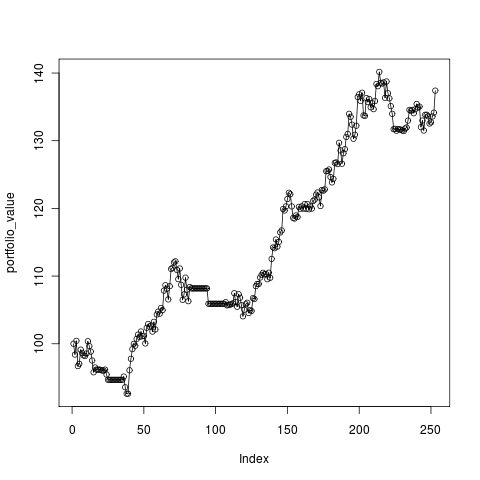
\includegraphics[scale=.4]{rplot0.png}
  \end{center}
  \caption{Chart shows value of portfolio in time}
  \label{fig:trend-short}
\end{figure}

There are easily visible periods of time (figure~\ref{fig:trend-short}) when the portfolio value is not changing. 
It is a time when our portfolio does not contain any assets (but we still have money). 
After a while conditions change and trend following algorithm decides to buy some assets.


\subsubsection{Intermediate-term trend results}

In this particular test (with values: $N = 20$, $M = 40$), trend following algorithm has been adjusted to focus on intermediate-term trends.
 
\begin{figure}[H]
  \begin{center}
    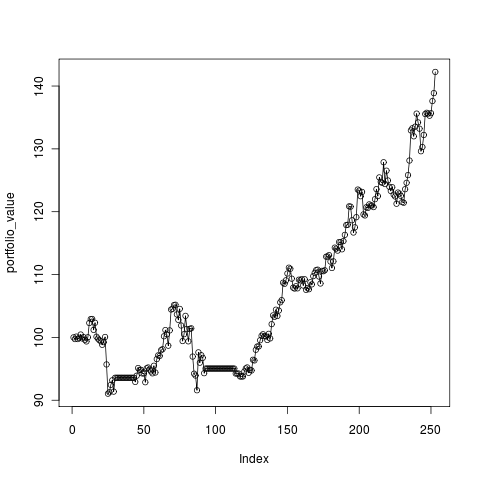
\includegraphics[scale=.4]{rplot.png}
  \end{center}
  \caption{Chart shows value of portfolio in time}
\end{figure}

\subsection{Conclusions}

It turned out that focusing on short-term or intermediate-term 

%---------------------------------------------------------------------------

\subsection{Genetic Algorithm}

\begin{figure}[H]
  \begin{center}
    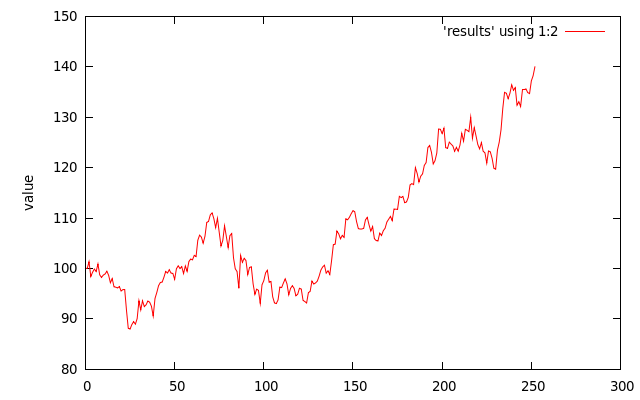
\includegraphics[scale=.5]{simple-genetic-algo.png}
  \end{center}
  \caption{GA flow chart \cite{Haupt:2004:PGA:1007746}}
\end{figure}


